%%%%%%%%%%%%%%%%%%%%%%%%%%%%%%%%%%%%%%%%%%%%%%%%%%%%%%%%%%%%%%%%%%%%%%%%%%%%%%%%
% AMS Beamer series / Bologna FC / Template
% Andrea Omicini
% Alma Mater Studiorum - Università di Bologna
% mailto:andrea.omicini@unibo.it
%%%%%%%%%%%%%%%%%%%%%%%%%%%%%%%%%%%%%%%%%%%%%%%%%%%%%%%%%%%%%%%%%%%%%%%%%%%%%%%%
%\documentclass[handout]{beamer}\mode<handout>{\usetheme{default}}
%
\documentclass[presentation]{beamer}\mode<presentation>{\usetheme{AMSBolognaFC}}
%\documentclass[handout]{beamer}\mode<handout>{\usetheme{AMSBolognaFC}}
%%%%%%%%%%%%%%%%%%%%%%%%%%%%%%%%%%%%%%%%%%%%%%%%%%%%%%%%%%%%%%%%%%%%%%%%%%%%%%%%
\usepackage[T1]{fontenc}
\usepackage{wasysym}
\usepackage{amsmath,blkarray}
\usepackage{centernot}
\usepackage{fontawesome}
\usepackage{fancyvrb}
\usepackage[ddmmyyyy]{datetime}
\usepackage{comment}
\usepackage{listings}
%!TeX root = paper-2023-coordination-marl-tool.tex

\lstdefinelanguage{scala}{
  keywords={abstract,case,catch,class,def,%
    do,else,extends,false,final,finally,%
    for,if,implicit,import,match,mixin,%
    new,null,object,override,package,%
    private,protected,requires,return,sealed,%
    super,this,throw,trait,true,try,lazy,%
    type,val,var,while,with,yield,forSome},
  otherkeywords={=>,<-,<\%,<:,>:,\#},
  sensitive=true,
  columns=fullflexible,
  morecomment=[l]{//},
  morecomment=[n]{/*}{*/},
  morestring=[b]",
  stringstyle=\ttfamily\color{red!50!brown},
  showstringspaces=false,
  morestring=[b]',
  morestring=[b]""",
  basicstyle=\sffamily\lst@ifdisplaystyle\scriptsize\fi\ttfamily,
  emphstyle=\sffamily\bfseries\ttfamily
}
\definecolor{ddarkgreen}{rgb}{0,0.5,0}
\lstdefinelanguage{scafi}{
  frame=single,
  basewidth=0.5em,
  language={scala},
  keywordstyle=\color{blue}\textbf,
  commentstyle=\color{ddarkgreen},
  keywordstyle=[2]\color{red}\textbf,
  keywords=[2]{rep,nbr,foldhood,foldhoodPlus,aggregate,branch,spawn,mux,mid},
  keywordstyle=[3]\color{gray},
  keywords=[3]{Me,AroundMe,Everywhere,Forever}, %,@@,@@@
  keywordstyle=[4]\color{red}\textbf,
  keywords=[4]{in,out,rd},
  keywordstyle=[5]\color{violet},
  keywords=[5]{evolve,when,andNext,workflow,G,C,broadcast,gossip,dilate, gradient, distance},
  keywordstyle=[6]\color{orange},
  keywords=[6]{Available,Serving,Done,Waiting,Removing,None,Set}
}
\lstset{language=scafi}
\renewcommand{\dateseparator}{}
%\renewcommand{\thefootnote}{\fnsymbol{footnote}}
\newcommand{\version}{1}
\usepackage[
	backend=biber,
	%citestyle=authoryear-icomp,
	maxcitenames=1,
	bibstyle=alphabetic]{biblatex}

	\makeatletter

\addbibresource{bibliography.bib}
%%%%%%%%%%%%%%%%%%%%%%%%%%%%%%%%%%%%%%%%%%%%%%%%%%%%%%%%%%%%%%%%%%%%%%%%%%%%%%%%
\title[]
{Hybrid AI-based engineering of cyber-physical swarms}
%
\subtitle[Research Project Proposal]
{Research Project Proposal}
%
\author[\sspeaker{Domini}]
{\speaker{Davide Domini} \href{mailto:davide.domini@studio.unibo.it}{davide.domini@studio.unibo.it}}
%
\institute[DISI, Univ.\ Bologna]
{Department of Computer Science and Engineering - DISI\\\textsc{Alma Mater Studiorum} -- University of Bologna
\\[0.5cm]
\textbf{Ph.D. Programme in Computer Science And Engineering \\ Admission XXXIX Cycle}}

%
\renewcommand{\dateseparator}{/}
\date[\today]{\today}
%
%%%%%%%%%%%%%%%%%%%%%%%%%%%%%%%%%%%%%%%%%%%%%%%%%%%%%%%%%%%%%%%%%%%%%%%%%%%%%%%%
\begin{document}
%%%%%%%%%%%%%%%%%%%%%%%%%%%%%%%%%%%%%%%%%%%%%%%%%%%%%%%%%%%%%%%%%%%%%%%%%%%%%%%%

%/////////
\frame{\titlepage}
%/////////

%%===============================================================================
\section*{Outline}
%%===============================================================================

%%/////////
\frame[c]{\tableofcontents[hideallsubsections]}
%%/////////

%===============================================================================
\section{Introduction}
%===============================================================================

%/////////
\begin{frame}[c]{Introduction}
%/////////

\begin{block}{Cyber-Physical Swarms (CPSW)}
	\begin{itemize}
		\item A myriad devices that \emph{interact} with the environment and \emph{exchange} information 
			among themselves;
		\item A wide range of applied domains, including: smart cities \cite{zedadra2019swarm}, 
			swarm robotics \cite{brambilla2013swarm}, 
			large-scale IoT systems \cite{uslu2023role}, and more.
	\end{itemize}
\end{block}

\begin{alertblock}{Engineering approaches}
	\begin{itemize}
		\item Macro-programming: manually developing controllers 
			from a global perspective (e.g., \emph{Aggregate Computing} \footnote{\fullcite {viroli2018field}});
		\item AI: learn directly from experience and/or data 
			(e.g., \emph{Multi-Agent Reinforcement Learning} \cite{4445757} and 
			\emph{Graph Neural Networks} \cite{9046288});
		\item Open space for \emph{hybrid approaches}.
	\end{itemize}
\end{alertblock}

\end{frame}
%/////////


%===============================================================================
\section{State of the art}
%===============================================================================

% %/////////
% \begin{frame}[allowframebreaks]{Aggregate computing}
% %/////////
% \begin{columns}
% \begin{column}{0.55\textwidth}
% 	\begin{block}{Overview}
% 		\begin{itemize}
% 			\item \emph{Computational fields} \cite{mamei2004cofields, viroli2019distributed} as first-class abstractions;
% 			\item Programs as field transformations through \emph{field calculus} \cite{viroli2016higher}.
% 		\end{itemize}
% 	\end{block}
% \end{column}
% \begin{column}{0.45\textwidth}
% 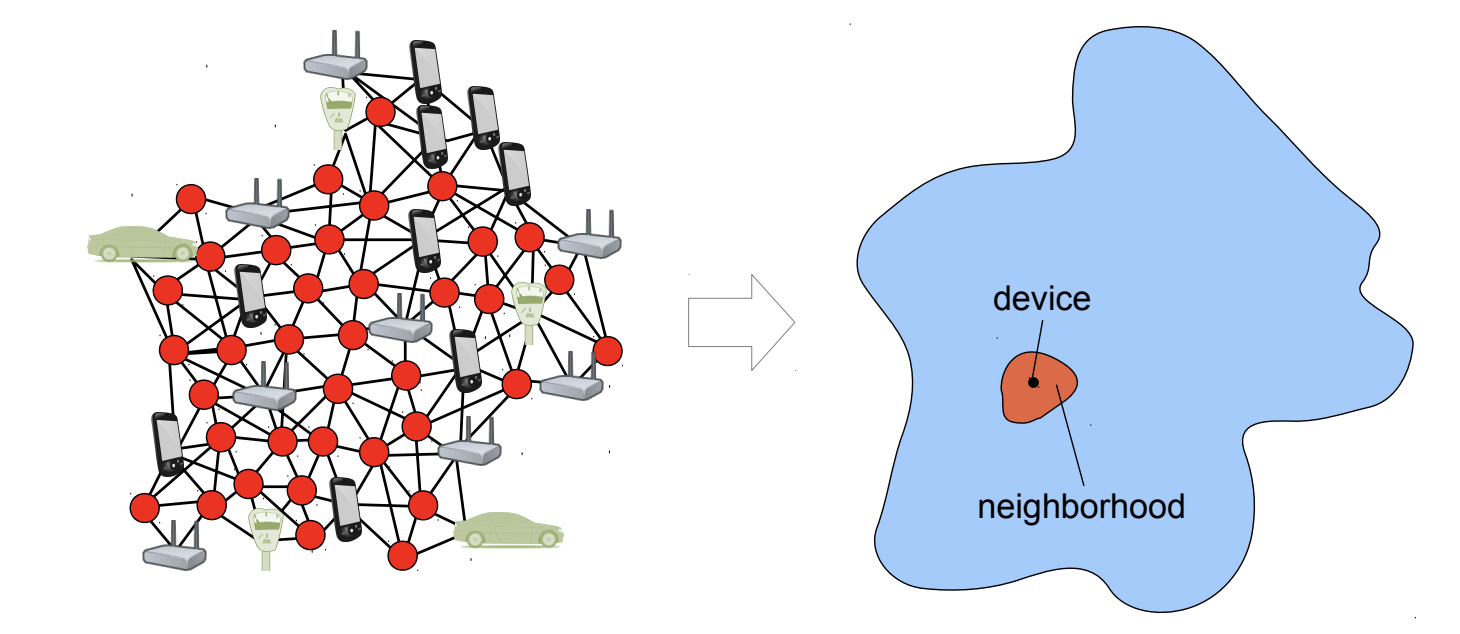
\includegraphics[width=\textwidth]{img/ac.png}
% \end{column}
% \end{columns}

% \centering
% \begin{alertblock}{Computational model}
% \begin{itemize}
% 	\item Each node shares the same \emph{aggregate program};
% 	\item Each node execute rounds iteratively and asynchronously:
% 	\begin{enumerate}
% 		\item \textbf{Sense}: collect information from the neighborhood and sensors;
% 		\item \textbf{Compute}: execute the aggregate program on the context;
% 		\item \textbf{Act}: share the export with the neighborhood.
% 	\end{enumerate}
% \end{itemize}
% \end{alertblock}

% \begin{alertblock}{Advantages}
% 	\begin{itemize}
% 		\item Programs defined in a \emph{composable} and \emph{declarative} manner;
% 		\item Promotes the \emph{reuse} of behaviours;
% 		\item Low-level aspects (e.g., failures) are \emph{automatically handled} by the middleware;
% 		\item A reliable and efficient Scala implementation: \emph{ScaFi} \cite{casadei2022scafi}
% 		\begin{itemize}
% 			\item A \emph{domain specific language (DSL)} for specifying aggregate computation;
% 			\item A \emph{simulation environment}, through the Alchemist simulator \cite{alchemist};
% 			\item A \emph{middleware} for executing and deploying aggregate programs;
% 			\item Reusable \emph{library functionalities} that serve as building blocks for constructing new aggregate
% 			programs (e.g., Gradients).
% 		\end{itemize}
% 	\end{itemize}
% \end{alertblock}

% \end{frame}
%/////////


%/////////
\begin{frame}[allowframebreaks, fragile]{Aggregate computing}
%/////////
\begin{columns}
	\begin{column}{0.55\textwidth}
		\begin{block}{Overview}
			\begin{itemize}
				\item \emph{Motto}: program the aggregate, not individual devices;
				\item \emph{Computational fields} \cite{mamei2004cofields, viroli2019distributed} as first-class abstractions;
				\item Programs as field transformations through \emph{field calculus} \cite{viroli2016higher}.
			\end{itemize}
		\end{block}
	\end{column}
	\begin{column}{0.45\textwidth}
	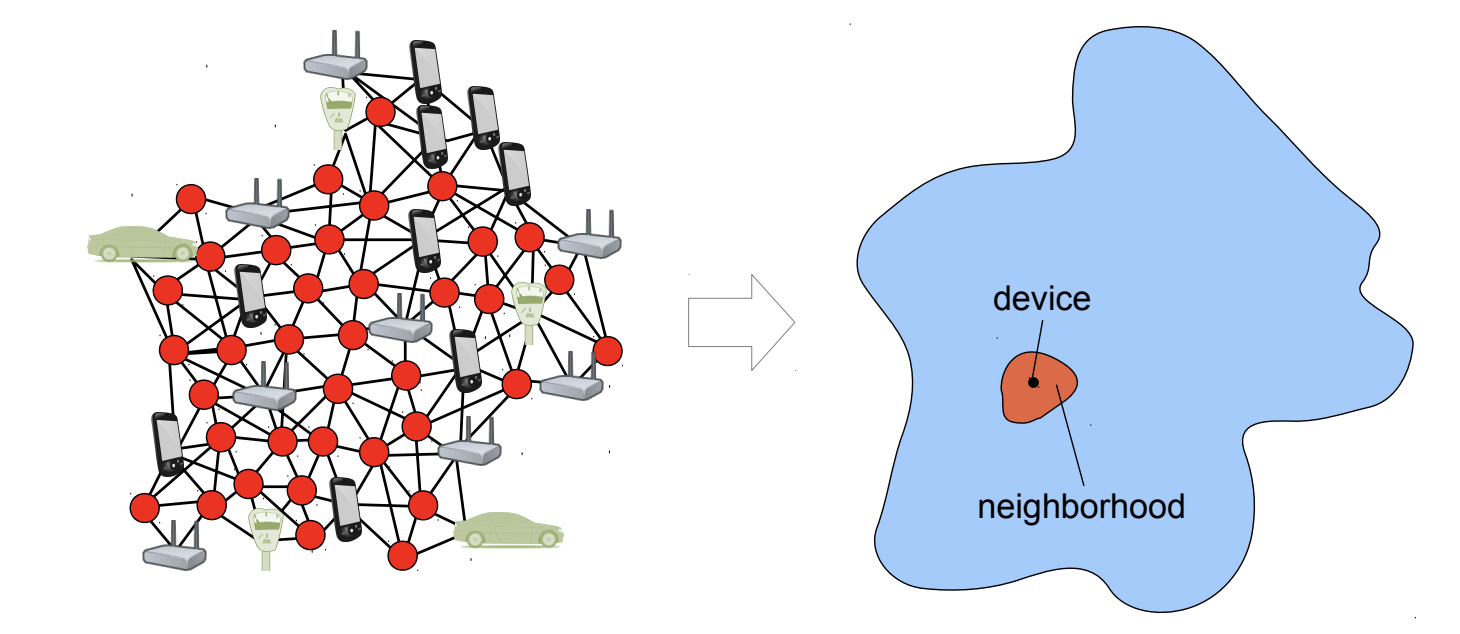
\includegraphics[width=\textwidth]{img/ac.png}
	\end{column}
\end{columns}
	
\centering

\begin{alertblock}{Advantages}
	 	\begin{itemize}
	 		\item Programs defined in a \emph{composable} and \emph{declarative} manner;
	 		\item Promotes the \emph{reuse} of behaviours;
	 		\item Low-level aspects (e.g., failures) are \emph{automatically handled} by the middleware;
	 	\end{itemize}
\end{alertblock}

\begin{columns}
	\begin{column}{0.5\textwidth}
		\begin{exampleblock}{Pratical example: the channel}
			\begin{itemize}
				\item We want a \emph{channel} from a given source to a given destination;
				\item Here the \emph{aggregate} nature of our approach gets revealed.
			\end{itemize}
		\end{exampleblock}
	\end{column}
	\begin{column}{0.5\textwidth}
		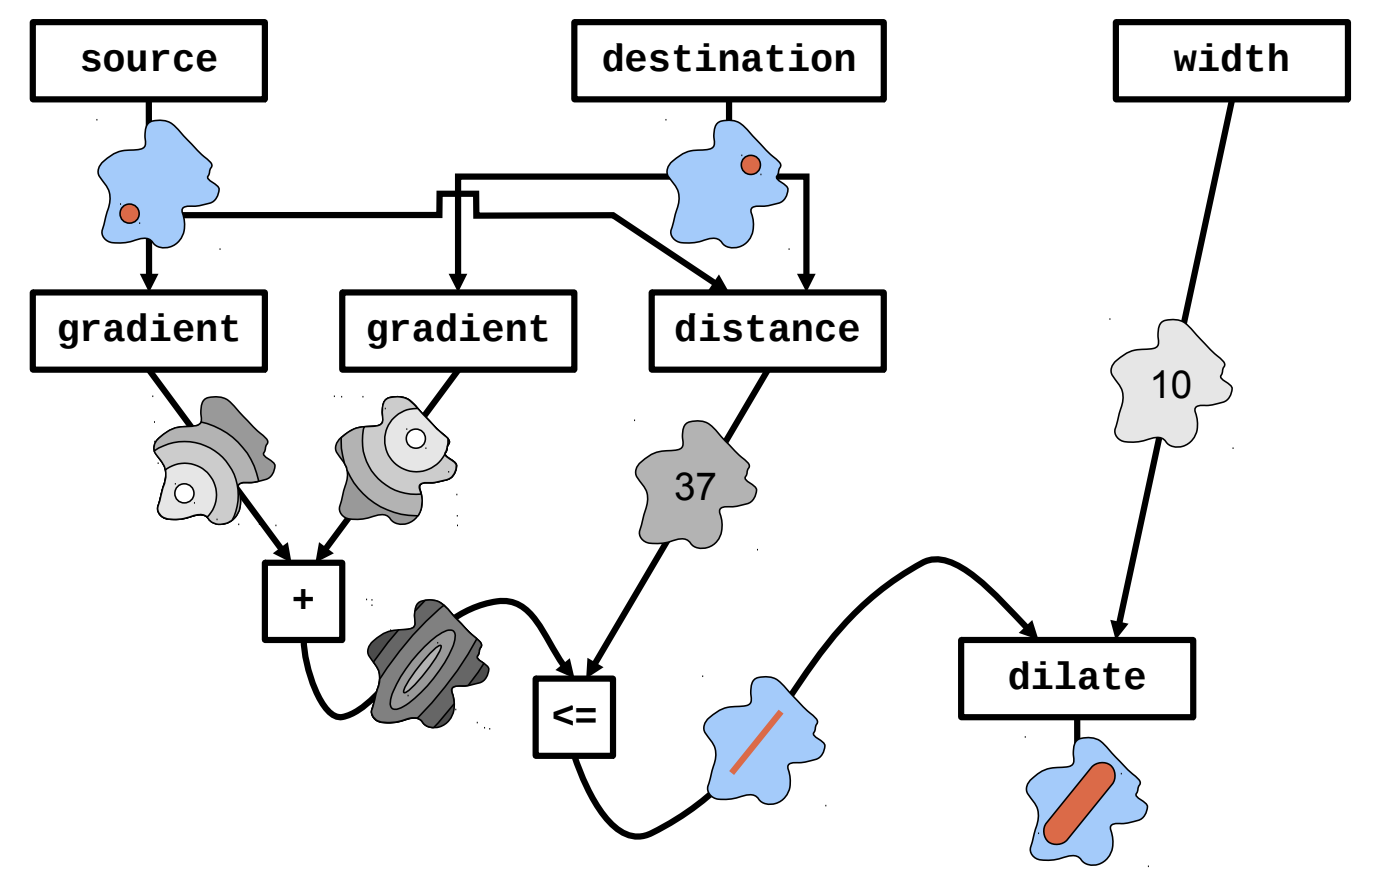
\includegraphics[width=\textwidth]{img/channel.png}
	\end{column}
\end{columns}

\centering

\begin{lstlisting}
def channel(source: Boolean, dest: Boolean, width: Double): Double {
   dilate(gradient(source) + gradient(dest) <= distance(source,dest), width)
}
\end{lstlisting}

\end{frame}
%/////////


%/////////
%\begin{frame}[allowframebreaks]{Learning from experience}
%/////////
% \begin{block}{Reinforcement learning}
% 	\begin{itemize}
% 		\item An \emph{agent} interacts with an \emph{environment} through \emph{actions};
% 		\item The environment provides a feedback signal (i.e., the \emph{reward});
% 		\item Agent goal: learn the optimal \emph{policy} to maximize some long-run measure of reinforcement.
% 	\end{itemize}
% \end{block}

% \centering
% 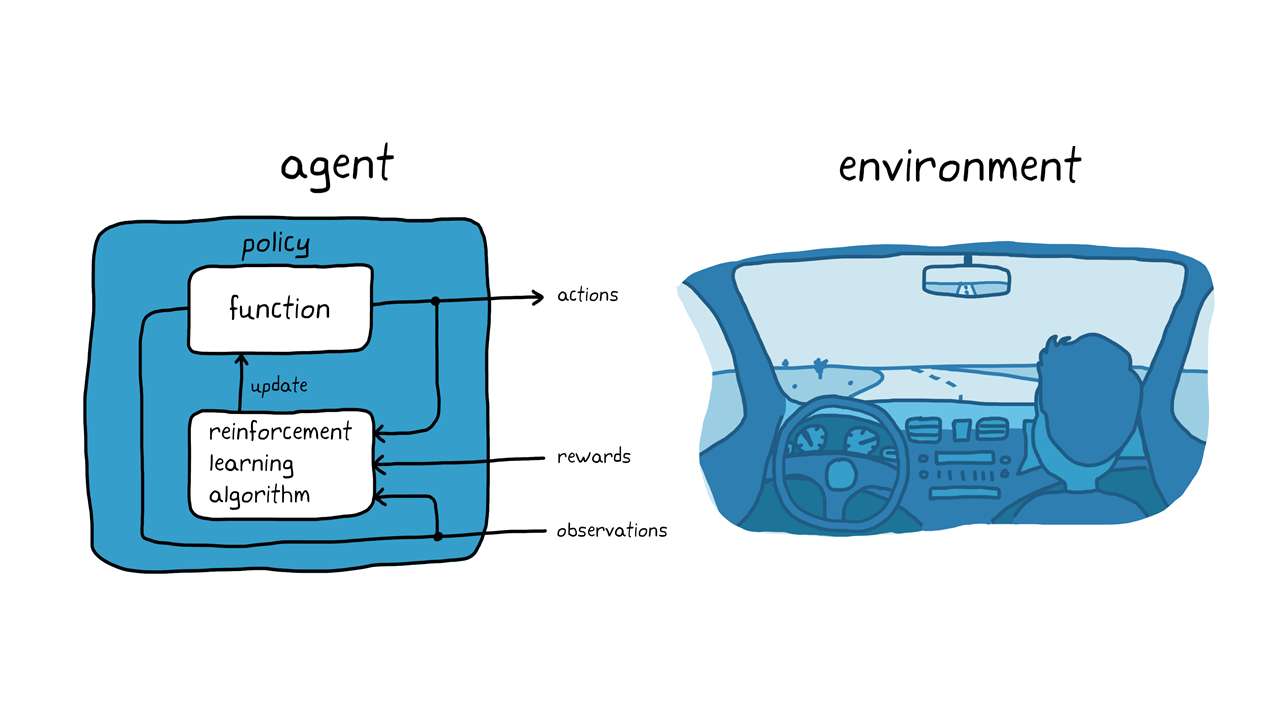
\includegraphics[width=0.6\textwidth]{img/rl.png}

% \begin{alertblock}{Algorithms}
% 	\begin{itemize}
% 		\item \textbf{Value-based}: aim to learn a value function that evaluates the goodness of each possible action from every 
% 				state in the environment (e.g., \emph{Q-Learning} \cite{dayan1992q}, \emph{DQN} \cite{mnih2013playing});
% 		\item \textbf{Policy-based}: aim to directly learn a behavioural policy (i.e., a state-action mapping) without
% 			utilizing an intermediate value function (e.g., \emph{Proximal Policy Optimization (PPO)} \cite{schulman2017proximal}).
% 	\end{itemize}
% \end{alertblock}

% \begin{alertblock}{Multi-Agent Reinforcement Learning}
% 	\begin{itemize}
% 		\item Extension of classic RL to multi-agent systems;
% 		\item Very promising field, but it introduces several challenges that need to be addressed, for example:
% 			 non-stationarity and equilibrium among the various policies.
% 	\end{itemize}
% \end{alertblock}

% \begin{alertblock}{Training mode}
% 	Based on information available to agents during training and execution phases we can classify 
% 		MARL algorithms into three families:
% 	\begin{itemize}
% 		\item Centralized Training and Centralized Execution (CTCE);
% 		\item Decentralized Training and Decentralized Execution (DTDE);
% 		\item Centralized Training and Decentralized Execution (CTDE).
% 	\end{itemize}
% \end{alertblock}

% \begin{alertblock}{Tasks}
% 	\begin{itemize}
% 		\item \textbf{Cooperative}: agents cooperate to maximize a global reward (we focus on this);
% 		\item Competitive: agents compete to maximize their own reward;
% 		\item Mixed: agents cooperate and compete at the same time.
% 	\end{itemize}
% \end{alertblock}

% \end{frame}
%/////////



%/////////
\begin{frame}[c]{Learning from experience}
%/////////

\begin{block}{Reinforcement learning}
	\begin{itemize}
		\item An \emph{agent} interacts with an \emph{environment} through \emph{actions};
		\item The environment provides a feedback signal (i.e., the \emph{reward});
		\item Agent goal: learn the optimal \emph{policy} to maximize some long-run measure of reinforcement.
	\end{itemize}
\end{block}


\begin{columns}
	\begin{column}{0.5\textwidth}
		\begin{alertblock}{Multi-Agent RL}
			\begin{itemize}
				\item Extension of classic RL to \emph{multi-agent systems};
				\item Very promising field;
				\item Several challenges need to be addressed (e.g., equilibrium).
			\end{itemize}
		\end{alertblock}
	\end{column}
	\begin{column}{0.5\textwidth}
		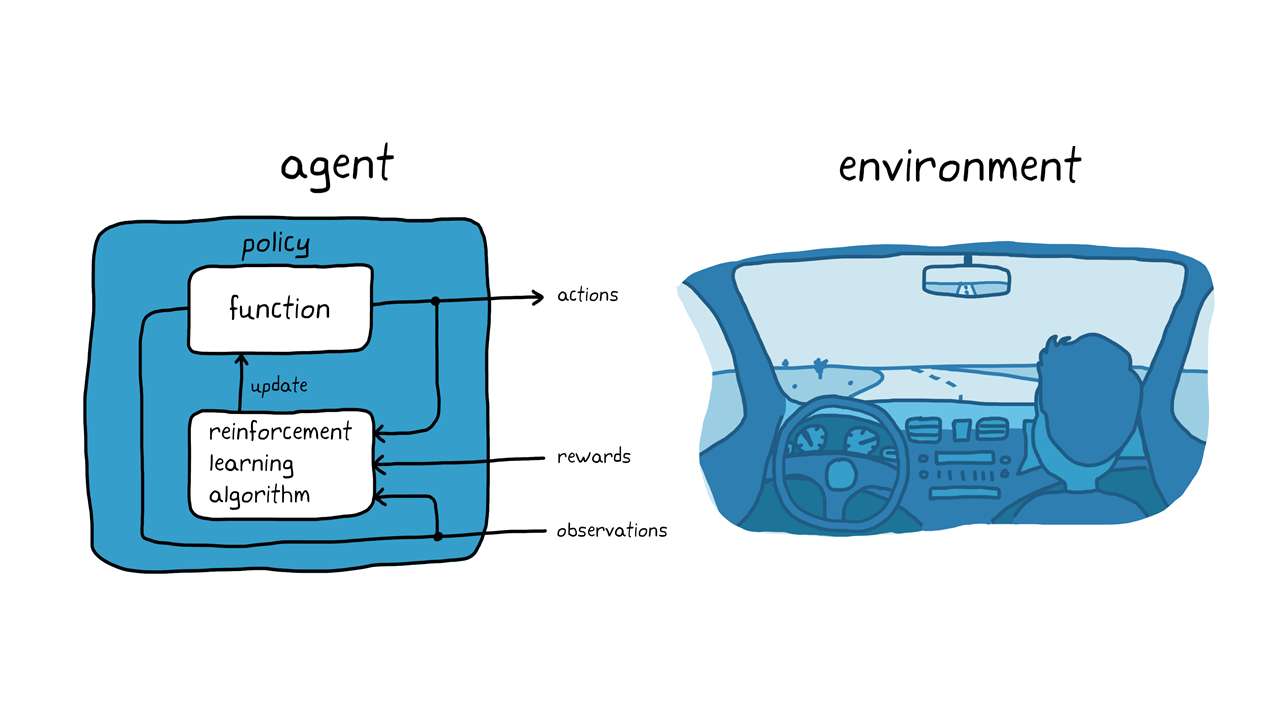
\includegraphics[width=\textwidth]{img/rl.png}
	\end{column}
\end{columns}


\end{frame}
%/////////

%/////////
\begin{frame}[c]{Graph Neural Networks}
%/////////

\begin{block}{Why}
	\begin{itemize}
		\item Nowdays data represented as \emph{graphs} are ubiquitous 
			(e.g., social networks, molecules in chemistry, etc.);
		\item \emph{Computational fields} can also be seen as graphs;
		\item This model can be \emph{distributed} across various nodes and applied to each of them, 
			as it only applies local transformations.
	\end{itemize}
\end{block}

\begin{columns}
	\begin{column}{0.5\textwidth}
		\begin{alertblock}{Many types of tasks}
			\begin{itemize}
				\item Node classification/regression;
				\item Edge classification/regression;
				\item Graph classification/regression;
				\item Node embeddings;
				\item Robotics.
			\end{itemize}
		\end{alertblock}
	\end{column}
	\begin{column}{0.5\textwidth}
		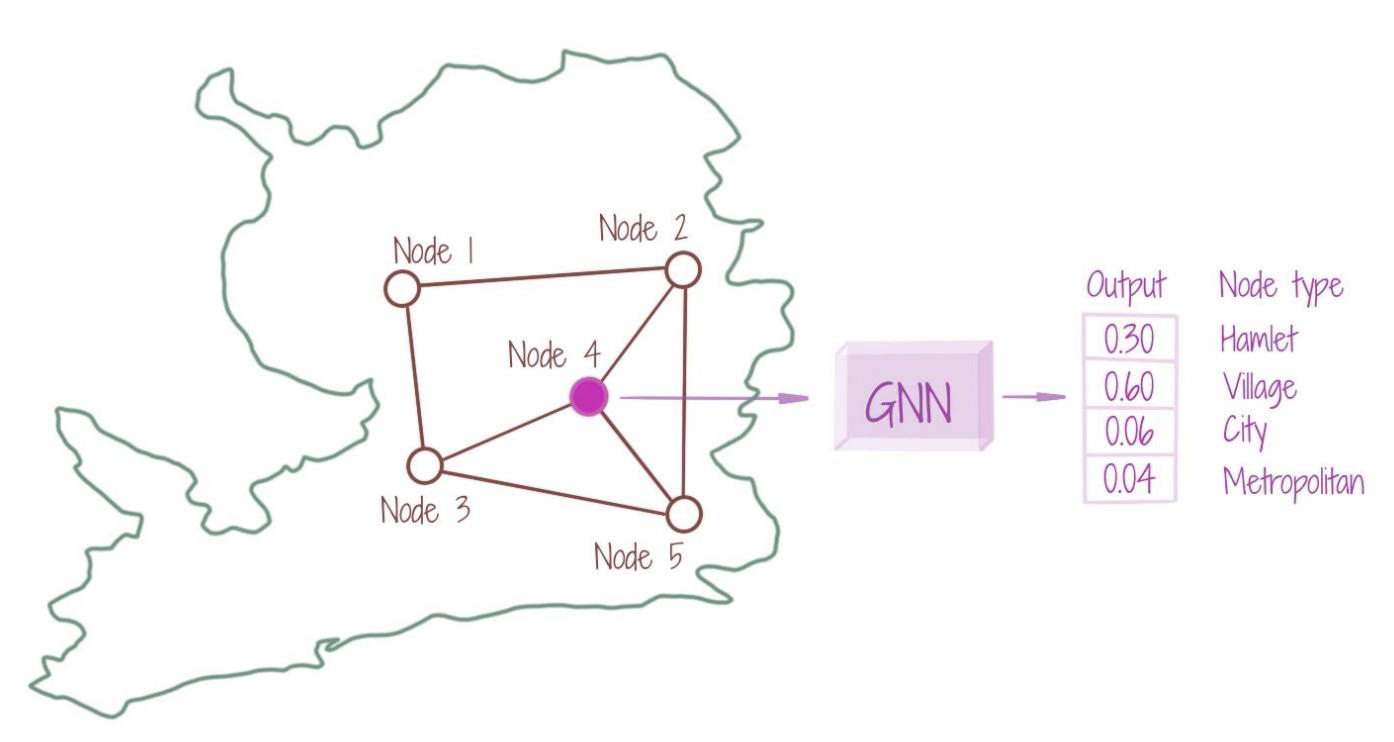
\includegraphics[width=\textwidth]{img/gnn.png}
	\end{column}
\end{columns}

% \begin{alertblock}{Computational model}
% 	\begin{itemize}
% 		\item There exists multiple variants of GNNs, but they all share the same basic structure composed of two phases;
% 		\item \textbf{Aggregate}
% 		\begin{itemize}
% 			\item Aggregation of information from neighbours;
% 			\item Usually, it is a simple function that performs a graph convolution on the neighbours;
% 		\end{itemize}
% 		\item \textbf{Combine}
% 		\begin{itemize}
% 			\item Combination of the aggregated information with the information present in the 
% 				node at the previous time step;
% 			\item Usually, it is a a differentiable complex function, such as a layer of a neural network.
% 		\end{itemize}
% 	\end{itemize}
% \end{alertblock}

\end{frame}
%/////////



%===============================================================================
\section{Project description}
%===============================================================================

%/////////
\begin{frame}[c]{Project description}

\begin{block}{Problems}
	\begin{itemize}
		\item CPSW \emph{coordination} to perform complex tasks, manually developing controllers 
			has some drawbacks:
		\begin{itemize}
			\item It is highly challenging to write satisfactory and efficient programs;
			\item Programs may be error-prone and lack of generality;
			%\item Programs may 
		\end{itemize}
		\item AI approaches also present challenges 
			(e.g., non-stationarity);
		%, for example:
		%\begin{itemize}
		%	\item Non-stationarity;
		%	\item Communication;
		%	\item Scalability.
		%\end{itemize}
	\end{itemize}
\end{block}
	
\begin{alertblock}{Proposed approach}
	\begin{itemize}
		\item \emph{Hybrid approach}: combination of aggregate computing and AI;
		\item Achieve a \emph{toolchain} that enables agile development of these systems;
		\item Advantages:
		\begin{itemize}
			\item Reducing the complexity of learning;
			\item Improving the adaptability of proposed solutions;
			\item Guiding the learning of complex behaviours in a simpler way through the use of 
				computational fields.
		\end{itemize}
	\end{itemize}
\end{alertblock}

\end{frame}
%/////////

%/////////
\begin{frame}[c]{Activities}

\begin{block}{Necessary steps}
	\begin{itemize}
		\item Define how \emph{learning of behaviours} can be pursued for CPSWs. 
			Two main possible approaches:
			\begin{itemize}
				\item Using aggregate computing to encode the information that will then be 
					passed to machine learning algorithms;
				\item Using machine learning to generate portions of aggregated programs;
			\end{itemize}
		\item Development of the \emph{toolchain} (already started with \emph{Scarlib}~\footnote{\fullcite{scarlib}})%\cite{scarlib});
		\item \emph{Benchmark}: selection of well-known examples from the state-of-the-art (e.g., flocking) 
			that will be used to evaluate the performance and usability of the toolchain;
		\item Opportunistic \emph{deployment}.
	\end{itemize}
\end{block}
	
\end{frame}
%/////////

%/////////
% \begin{frame}[c]{Scope}

% \begin{block}{Scope}
% 	\begin{itemize}
% 		\item \emph{Distributed AI}: integration with CPSW will bring forth several challenges that contribute
% 		to this field, for example:
% 		\begin{itemize}
% 			\item Continuous learning: ensure that agents can not only learn during the initial phase but also
% 				refine their knowledge online once they have been deployed;
% 		\end{itemize}
% 		\item \emph{Swarm robotics}: automatic design of controllers for swarm of robots;
% 		\item \emph{Software engineering}: development of novel models, 
% 			design techniques, languages, and algorithms that can be utilized to
% 			effectively handle the complexity of CPSW.
% 	\end{itemize}
% \end{block}


%\end{frame}
%/////////

%/////////
%\begin{frame}[c]{Technology}
%TODO ?	
	
%\end{frame}
%/////////


%/////////
\begin{frame}[c]{Expected results}

% \begin{block}{One year goal}
% 	\begin{itemize}
% 		\item Analysis of state-of-the-art AI techniques
% 			for the domain of CPSW;
% 		\item Hybrid tool-chain: integration of AC and AI in simulation and with
% 		offline learning;
% 		\item Implementation of custom RL and GNNs models
% 		and algorithms.
% 	\end{itemize}
% \end{block}

\begin{block}{PhD goal}
	\begin{itemize}
		\item Hybrid tool-chain;
		%\begin{itemize}
		%	\item Opportunistic deployment;
		%	\item Online learning; 
		%	\item Continuous learning to refine agents knowledge;
		%\end{itemize}
		\item Privacy: management of learning with sensitive data 
			(e.g., through federated learning);
		\item Development of application examples using the new platform.
	\end{itemize}
\end{block}

\begin{alertblock}{Long term contributions}
	\begin{itemize}
		\item Bridge the worlds of symbolic and sub-symbolic AI;
		\begin{itemize}
			\item Computational fields can be interpreted as a symbolic model 
				of the surrounding environment and interactions among agents;
		\end{itemize}
		\item Understand the extent to which these CPSWs can 
			become mainstream in modern contexts, such as:
		\begin{itemize}
			\item Large-scale IoT and Industry 4.0;
			%\item Industry 4.0;
			\item Swarms of robots for exploring inhospitable environments for humans.
		\end{itemize}
	\end{itemize}
\end{alertblock}

\end{frame}
%/////////

%/////////
% \begin{frame}[c]{Expected results II}

% \begin{alertblock}{Long term contributions}
% 	\begin{itemize}
% 		\item Bridge the worlds of symbolic and sub-symbolic AI;
% 		\begin{itemize}
% 			\item Computational fields can be interpreted as a symbolic model 
% 				of the surrounding environment and interactions among agents;
% 		\end{itemize}
% 		\item Understand the extent to which these CPSWs can 
% 			become mainstream in modern contexts, such as:
% 		\begin{itemize}
% 			\item Large-scale IoT;
% 			\item Industry 4.0;
% 			\item Swarms of robots for exploring inhospitable environments for humans.
% 		\end{itemize}
% 	\end{itemize}
% \end{alertblock}

% \end{frame}

%===============================================================================
\section*{}
%===============================================================================

%/////////
\frame{\titlepage}
%/////////

%===============================================================================
\section*{\refname}
%===============================================================================

%%%%
\setbeamertemplate{page number in head/foot}{}
%/////////
\begin{frame}[c,noframenumbering, allowframebreaks]{\refname}
%\begin{frame}[t,allowframebreaks,noframenumbering]{\refname}
	\tiny
	\nocite{*}
	\printbibliography
\end{frame}
%/////////

%%%%%%%%%%%%%%%%%%%%%%%%%%%%%%%%%%%%%%%%%%%%%%%%%%%%%%%%%%%%%%%%%%%%%%%%%%%%%%%%
\end{document}
%%%%%%%%%%%%%%%%%%%%%%%%%%%%%%%%%%%%%%%%%%%%%%%%%%%%%%%%%%%%%%%%%%%%%%%%%%%%%%%%
